%=============================================================================%
%                                 Preamble                                    %
%=============================================================================%
\documentclass[12pt,a4paper]{article}
%=============================================================================%
%							PACKAGE											  %
%=============================================================================%
\usepackage[french]{babel} % langue
\usepackage[utf8]{inputenc} % encodage
\usepackage{a4} % format
\usepackage{setspace} % interligne
\onehalfspacing % définit un interligne de 1.5
\usepackage[T1]{fontenc}
\usepackage[cyr]{aeguill}
\usepackage{epsfig}
\usepackage{amsmath, amsthm}
\usepackage{amsfonts,amssymb}
\usepackage{float}

%=============== changement de la numérotation des section ect...=============%
% \renewcommand{\thesection}{\Alph{section}}  % ex: ici les section sont définis avec des lettre
% \Alph --> Lettre	;	\Roman --> chiffre romain
%============================= couleur texte =================================%
\usepackage{xcolor}
\definecolor{green2}{rgb}{0,0.6,0}
\definecolor{grey2}{rgb}{0.4,0.4,0.4}

%============================ lien hypertext =================================%
\usepackage{hyperref}	
%utilisation href{url}{texte contenant le lien hypertext}

%============================ marge document =================================%
\usepackage{geometry}
\geometry{hmargin = 2.5cm, vmargin = 2.5cm}

%============================ mode paysage ===================================%
\usepackage{lscape} % page en paysage

%=============================== En-têtes et pied de page ====================%
\usepackage{fancyhdr}
\pagestyle{fancy} % est un style de page.
\usepackage{lastpage}
\renewcommand\headrulewidth{1pt}
\fancyhead[R]{Gestion informatique des données de séquençage}
\fancyhead[L]{M1 BI-IPFB Université de Paris}
\renewcommand\footrulewidth{1pt}
\fancyfoot[l]{William Amory}
\fancyfoot[c]{\textbf{Page \thepage/\pageref{LastPage}}}
\fancyfoot[r]{\today}
%=============================================================================%
%					    	Titre - Auteur - Date	        	 		      %
%=============================================================================%
\title{Gestion informatique des données de séquençage \\ Genoscope - LBGB}
\author{William Amory \\ M1 BI-IPFB Université Paris Cité \\\\ sous la responsabilité de Frédérick Gavory}
\date{\today}
%=============================================================================%
%						        Début document   							  %
%=============================================================================%
\begin{document}

%=============================================================================%
%                             Page de Garde                                   %
%=============================================================================%
\begin{titlepage}

    \newcommand{\HRule}{\rule{\linewidth}{0.5mm}} % nouvelle cmd pour tracer de lignes horizontale
  
    \begin{figure}[ht!]
        
\includegraphics[width=0.15\linewidth]{img/cea.jpg}
        \hspace{6cm}
        
\includegraphics[width=0.5\linewidth]{img/genoscope_logo.png}
    \end{figure}
    \vspace{1cm}
  
    \begin{center}
  
  %	HEADING SECTION
        \textsc{\LARGE Laboratoire de Bioinformatique pour la Génomique et la Biodiversités}\\[1cm]
        \Large{ Master de bioinformatique - ingénierie de plate-forme en biologie \\ \textsc{Univesité de Paris}}\\[0.2cm]
  
  
  %	TITLE SECTION
        \vspace{1cm}
        \HRule \\[0.4cm]
        {\huge Rapport d'alternance}\\[0.2cm]
        {\Huge \bfseries Gestion informatique des \\ données de séquençage}\\
        \HRule \\[1cm]

        \LARGE{\textbf{\today}} \\[1cm]

        \LARGE{William Amory}\\
        \LARGE{sous la resposabilité de Frédérick Gavory}\\[1cm]
    
    \end{center}
  
    \begin{figure}[ht!]
        
\includegraphics[width=0.4\linewidth]{img/logo}
    \end{figure}
    %\vfill % Fill the rest of the page with whitespace
    \newpage
  
\end{titlepage}
%\maketitle % afficher titre
% \addtocontents{toc}{\protect\thispagestyle{empty}} % toc non numéroté
{\hypersetup{hidelinks}
    \tableofcontents}
% \tableofcontents % affiche la toc
% \thispagestyle{empty} % suprime le style de la page
% \setcounter{page}{1} % numérote cette page comme la 1ere

%=============================================================================%
%                                 Contenu                                     %
%=============================================================================%
\newpage
\section*{Glossaire}

\begin{description}
    \item[BGI : ] \emph{Beijing Genomics Institute}, est une entreprise Chinoise de biotechnologie fondé en 1999.
    \item[CEA :] Commissariat à l'Énergie Atomique et aux Énergies Alternatives
    \item[CNRGH :] Centre National de Recherche en Génomique Humaine 
    \item[CNS :] Centre National de Séquençage (Genoscope)
    \item[CPU :] \emph{Central Processing Unit} (Unité Central de Traitement)
    \item[DNB :] \emph{DNA-nanoballs} (Nano \og billes\fg{} d'ADN générés lors de l'amplification ADN pour les séquenceurs de la technologie MGI)
    \item[DRF :] Direction de la Recherche Fondamentale
    \item[ERGA] \emph{European Reference Genome Atlas}
    \item[IBFJ :] Institut de Biologie François Jacob
    \item[Illumina :] Entreprise Californienne de biotechnologie fondée en 1998, qui réalise : R\&D, production et vente d’instruments de séquençage d’ADN à haut débit et très haut débit, ainsi que des logiciels et services d'analyses bio-informatique des données de séquençage.
    \item[Jira :] Logiciel de gestion de projet, de suivi d'incidents et de bugs développé par l'entreprise Atlassian
    \item[LBGB :] Laboratoire de Bioinformatique pour la Génomique et la Biodiversité
    \item[Lims :] \emph{Laboratory Information Management System}
    \item[MGI : ] Filiale du groupe BGI fondée en 2016 dont les missions sont : R\&D, production et vente d’instruments de séquençage 
    d’ADN, de réactifs et de produits connexes
    \item[NCBI :] \emph{National Center for Biotechnologiy Information}, est un institut national des Etats Unis d'Amériques pour l'information biologique moléculaire. Il développe notamment la base de données de génomes GenBank et la base de données des publications PubMed
    \item[NGL :] \emph{Next Generation LIMS} (bases de données du Genoscope et du CNRGH)
    \item[NGL\_BI :] \emph{NGL Bioinformatic} (base de données des analyses et traitements bio-informatique)
    \item[NGL\_PROJECT :] \emph{NGL projects} (base de données des projets en cours et passé)
    \item[NGL\_REAGENT :] \emph{NGL reagent} (base de données des réactifs)
    \item[NGL\_SEQ :] \emph{NGL Sequencing} (base de données de suivi des échantillons)
    \item[NGL\_SUB :] \emph{NGL submission} (base de données des soumissions de projet ou d'articles (exemple : la soumission d'un projet au NCBI))
    \item[NGS :] \emph{Next Generation Sequencing}
    \item[NGS\_BA :] \emph{Next Generation Sequencing - biological analysis}
    \item[NGS\_QC] \emph{Next Generation Sequencing - quality control}
    \item[NGS\_RG : ] \emph{Next Generation Sequencing - reads generation}
    \item[Oxford Nanopore :] Entreprise Anglaise de biotechnologie fondée en 2005, qui développe et produit des systèmes de séquençage, basé sur les propriété diélectrique de ces dernières.
    \item[PacBio :] \emph{Pacific Biosciences of California} est une entreprise Californienne fondée en 2004, qui développe et produit des systèmes de séquençage en temps réel à molécule unique (SMRT) d'ADN
    \item[Path : ] Chemin d'accès à un fichier ou à un répertoire dans le système de fichier
    \item[Perl :] \emph{Pratical Extraction and Report Language}
    \item[Ram :] \emph{Random Access Memory} (Accès Mémoire Aléatoire, aussi appelé mémoire vive)
    \item[Slurm :] \emph{Simple Linux Utility for Resource Management} qui est un logiciel open source d'ordonnancement des tâches informatiques
\end{description}
\addcontentsline{toc}{section}{Glossaire}

\newpage
\section{Introduction}
\subsection{LBGB au sein du Genoscope et du CEA}
Le Genoscope (CNS) a été créé en 1996 pour participer au projet mondial de séquençage du génome humain (\emph{Human Genome Project}) qui à débuté en 1990 et s'est terminé en 2003. Il a notament participé au séquençage du chromosome 14. Le Genoscope est impliqué dans le développement de programme de génomique en France dans le cadre du projet France génomique. Aujourd'hui les projets phares du Genoscope sont les projets \textbf{Tara} (\emph{Pacific}, Océans, \emph{Artic} ...), qui ont pour objectifs l'étude des écosystèmes marins ; Le projet \textbf{ERGA}, dont l'objectif est de créer une base de données de références de haute qualité des génomes d'espèces européennes.

\begin{minipage}{0.45\textwidth}
\begin{figure}[H]
    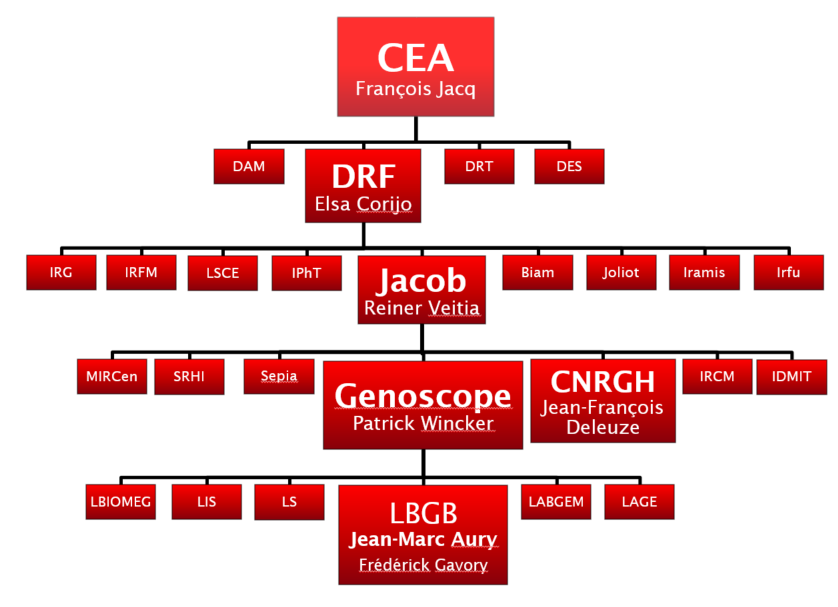
\includegraphics[width=1.1\textwidth]{img/organigramme.png}
    \caption{Organigramme situant l’équipe du LBGB au sein du Genoscope et du CEA}
    \label{organigramme_LBGB}
\end{figure}
\end{minipage} 
\hfill
\begin{minipage}{0.45\textwidth}
    Le Laboratoire de Bioinformatique pour la Génomique et la Biodiversité (\textbf{LBGB}) dirigé par Jean-Marc Aury, fait partie du Genoscope qui est une composante de l'institut de biologie François Jacob (\textbf{IBFJ}) de la direction de la recherche fondamentale (\textbf{DRF}) du Commissariat à l'Énergie Atomique et aux Énergies Alternatives (\textbf{CEA}), qui a été fondé le 18 octobre 1945 par Charles de Gaulle. L'intégration du genoscope au CEA a été réalisée en 2007, et en 2017 il devient une composante de l'IBFJ.
\end{minipage}

\subsection{Contexte et missions du LBGB}
Les missions qui sont confiées au LBGB sont de réaliser le contrôle qualité des données de séquences issues des différents séquenceurs, d'effectuer l'assemblage\footnote{Reconstruction d'un génome à partir de fragments de ce dernier} des séquences et l'annotation\footnote{Documenter le plus exhaustivement possible les informations de l'assemblage permmettant de prédire la fonction d'une molécule} des génomes, dans l'objectif de mettre à disposition des laboratoires collaborateurs les données avec un premier niveau da valorisation. Le laboratoire est divisé en plusieurs groupes de travail. Le groupe \og production \fg{} (dont je fais partie), le groupe \og assemblage \fg{}, le groupe \og annotation \fg{} et le groupe \og évaluation des technologies de séquençage \fg{}.

Les missions du groupe de \og production \fg{} sont de tester des logiciels tiers, de développer et maintenir des scripts utilisant ces logiciels pour gérer efficacement la prise en charge des données en sortie de séquençeur. Cette prise en charge peut répondre à une demande de la production et des laboratoires du Genoscope et du CNRGH, mais aussi pour des laboratoires extérieurs. L'objectif principale est la mise en place et le maintient de pipelines automatisant l'ensemble. Le groupe s'appuie sur un travail de veille et d'évaluation technologique pour chacune de ses missions. 


\subsection{Présentation du workflow NGS}
\begin{minipage}{0.45\textwidth}
	\begin{figure}[H]
		\centering
		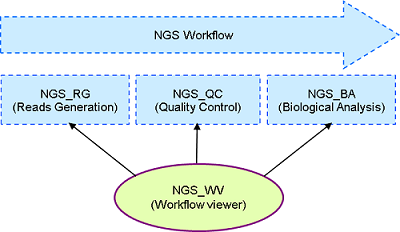
\includegraphics[width=1\textwidth]{img/Workflow.png}
		\caption{\footnotesize{Workflow de génération, de contrôle qualité et d’analyse biologique des fastq}}
		\label{worflow-genoscope}
	\end{figure}
\end{minipage}
\hfill
\begin{minipage}{0.45\textwidth}
	Le workflow NGS est composé de trois pipelines pour les technologies Illumina et Oxford Nanopore. Le premier (ngs\_rg\footnote{\emph{Next Generation Sequencing - reads generation}}), permet la génération des reads\footnote{Lecture d'une séquence par un séquenceur d'un fragments d'ADN} et des fichiers de séquences correspondants aux échantillons. Le second (ngs\_qc\footnote{\emph{Next Generation Sequencing - quality control}}), permet de réaliser leur contrôle qualité. Le dernier (ngs\_ba\footnote{\emph{Next Generation Sequencing - biological analysis}}), permet de faire les analyses biologiques inter-échantillons (\emph{readset})\footnote{Un lot de séquences est une instance de séquences (ou reads) d'un échantillon}. 
\end{minipage}\\[0.1cm]

Ces trois pipelines sont automatisés dans le workflow et permettent de réaliser la distribution des données de séquençage, par projet, échantillon, runs\footnote{Séquençage d'un ou plusieurs échantillons sur un séquenceur} et technologie de séquençage. Ils réalisent aussi le nettoyage, l'analyse de ces fichiers et mettent à jour la base de données de référence NGL. Les trois pipelines du workflow NGS sont monitorés par NGS \emph{Worqflow Viewer} (NGS\_WV), qui est une application web permettant de surveiller l'avancement des pipelines pour les runs pris en charge par le NGS-workflow.

\subsection{La technologie MGI}
Le genoscope et le CNRGH ont récement fait l'aquisition de séquenceurs MGI (2 DNBSEQ-G400 et 1 DNBSEQ-T7).

\begin{minipage}{0.45\textwidth}
    \begin{figure}[H]
        \centering
        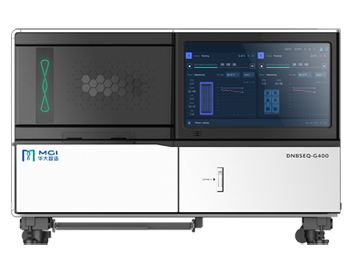
\includegraphics[width=0.5\textwidth]{img/MGI_G400.jpg}\\
        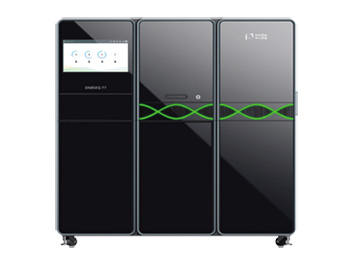
\includegraphics[width=0.5\textwidth]{img/MGI_T7.jpg}
        \caption{\footnotesize{Sequenceurs DNBSEQ-G400 (en haut) et DNBT7 (en bas) de MGI \href{https://en.mgi-tech.com/products/}{https://en.mgi-tech.com/products/}}}
        \label{seq-MGI}
    \end{figure}
\end{minipage} 
\hfill
\begin{minipage}{0.45\textwidth}
	\begin{figure}[H]
        \centering
        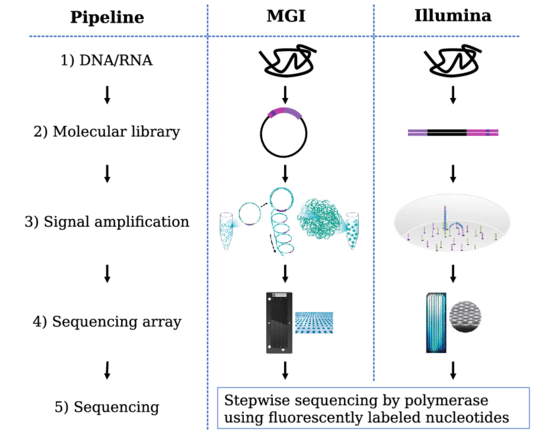
\includegraphics[width=1\textwidth]{img/MGI_vs_Illumina.png}
        \caption{\footnotesize{Différences entre Illumina et MGI de technologie NGS}}
        \label{fig-Illu-vs-MGI}
    \end{figure}
\end{minipage}\\\\

    Il s'agit de séquenceurs à haut débit et très haut débit, dont les principales différences entre MGI et Illumina sont dans la création des librairies\footnote{Collection de fragment d'ADN issue du génome complet d'un organisme ou plusieurs organismes (méta-génomique) et clonés dans un vecteur (le plus souvanet dans des plasmides)} et la méthode d'amplification d'ADN. Les librairies sont double brins circulaire pour MGI, alors que pour Illumina elle est double brins linéaire. L'amplification ADN est réalisée en solution et forme des DNB (\emph{DNA-nanoballs}\footnote{Nanobilles d'ADN générées par la réplication de l'ADN circulaire}), puis déposée sur la Flowcell\footnote{Lame d'absorbtion des fragments d'ADN et cuve réacteur du séquençage} pour MGI, alors que pour Illumina elle est réalisée après immobilisation sur les Flowcell.

\begin{table}[H]
\begin{tabular}{ |p{5cm}||r|r|r|r| }
    \hline
    \multicolumn{5}{|c|}{Sequencers specifications} \\\hline
    & \footnotesize{DNBSEQ-G400} & \footnotesize{DNBSEQ-T7} & \footnotesize{HiSeq 4000} & \footnotesize{NovaSeq 6000} \\\hline\hline
    Max Number of Flow Cells & 2 & 4 & 2 & 2 \\\hline
    Max Lane/Flow Cell & 4 & 1 & 4 & 4 \\\hline
    Run Time & $\sim$ 14-37 h & $\sim$ 20-30 h & $\sim$ 24-84 h & $\sim$ 13-44 h \\\hline
    \textbf{Data ouput/Run} & 0.27-1.4 Tb & 1-6 Tb & 0.9-1.8 Tb & 1-6 Tb \\\hline
    Max Reads/Run & 1.8 billions & 5 billions & 10 billions & 20 billions \\\hline
    Max Read Length & 2 $\times$ 200 bp & 2 $\times$ 150 bp & 2 $\times$ 150 bp & 2 $\times$ 250 bp \\\hline
\end{tabular}
    \caption{Spécification des séquenceurs}
    \label{spe-seq}
\end{table}

\section{Objectifs de ma mission}
L'objectif principal de ma mission est la mise en place d'un workflow NGS pour les séquenceurs MGI. Dans un premier temps il s'agira de créer un pipeline de génération de fichiers de séquences (NGS\_RG\_MGI\footnote{\emph{Next Generation Sequencing - reads generation - mgi}}) puis un pour le contrôle qualité de ces fichiers (NGS\_QC\_MGI\footnote{\emph{Next Generation Sequencing - quality control - mgi}}). Le workflow devra créer et mettre à jour l'état des runs, des pistes ou (\emph{lane}) et de readset\footnote{Lot de séquences} dans NGL, réaliser le contrôle qualité des fichiers de séquences, au format FASTQ, obtenus en fin de séquençage. Il devra mettre à jour l'avancement du traitement d'un run dans NGL, en y insérant les métriques et statistiques obtenues lors du démultipléxage\footnote{Séparation des séquences en plusieurs fichiers en fonction de leurs index (séquence d'une dizaines de nucléotides en amont du primer de la séquence)}, les résultats des contrôles qualités, etc. Puisque l'objectif est d'obtenir un premier niveau de valorisation des fichiers de séquences, permettant aux autres groupes (\og assemblage \fg{}, \og annotation \fg{}) de prendre en charge ces fichiers avant de les mettre à disposition des laboratoires collaborateurs.\\

Je dois également, rechercher et réaliser des évaluations de nouveaux outils pour les différents pipelines des différentes technologies de séquençage, en vue d'un potentiel ajout ou de remplacement d'outils. Il sera donc nécessaire de maintenir les pipelines des différentes technologies de séquençage en conséquence. Par exemple l'évaluation de logiciels de trimming (Cutadapt, Trimmomatic) en vue d'un remplacement du l'outil fastx\_clean de l'extension fastxend de la suite FASTX Toolkit\footnote{Collection de commandes pour le traitement et l'évaluation de lot de séquences au format FASTA ou FASTQ} qui est un outil mono-coeur pour un outil multi-coeurs. Ou bien trouver et évaluer un logiciel d'assignation taxonomique plus performant que le logiciel Centrifuge utilisé actuellement.
\section{Matériels et Méthodes}
\subsection{Le cluster de calcul et Slurm}
Le Genoscope possède un cluster (\emph{inti}) de calcul de 66 noeuds répartis sur 5 partition. La partition \og normal\fg{} est composé de 44 noeuds qui disposent entre 12 et 36 Go coeurs et entre 96 et 386 Go de ram. La partition \og small\fg{} est composé de 12 noeuds dont 4 qui possèdent 8 coeurs et 64 Go de RAM, et 4 autres qui disposent de 16 coeurs et 128 Go de RAM. Cette partition est utilisé pur les processus court et/ou peu de mémoire. Les partition \og xlarge \fg{} et \og xxlarge\fg{} ont deux noeuds composés de 48 et 2To de RAM, et de 56 coeurs et 6To de RAM respectivement. Ces deux partition sont utilisés pour les processus demandant plusieurs jours ou semaines de caluls.
La partition \og production\fg{} du cluster \emph{inti} est composé 12 noeuds qui disposent de 16 coeurs et de 257 Go de RAM.
L'accès à l'utilisation du cluster et de ses noeuds est réalisé par le logiciel Slurm.

\subsection{La base de données de référence NGL et la gestion des projets}
Le Genoscope dispose de sa propre base de données de référence NGL. Celle-ci est divisée en plusieurs parties. NGL\_BI\footnote{NGL Bioinformatic}, est la partie de la base de données utilisée par les équipes de bioinformatique. NGL\_SEQ\footnote{NGL Sequencing}, est la partie de la base de données utilisée dès la réception des échantillons et jusqu'au séquençage de ces derniers. Il y a également les parties NGL\_sub\footnote{NGL submission (base de données des soumissions de projet (example la soumission d'un projet au NCBI))}, NGL\_reagent\footnote{NGL reagent (base de données des réactifs)} et NGL\_projects\footnote{NGL projects (base de données des projets en cours et passé)}. La gestion et le suivi du développement informatique sont réalisés par le système de tickets Jira.

\subsection{Le langage de programmation Perl}
L'écriture du workflow des pipelines pour les séquenceurs MGI est réalisée dans le langage de programmation Perl. L'utilisation de ce langage est rendu necessaire pour des raisons historique du laboratoire, puisque de nombreuses librairies et modules qui ont été utilisés dans l'écriture des pipelines sont écrits en Perl.\\

C'est pour toutes ces raisons qu'il m'a été nécessaire d'apprendre à coder en Perl. j'ai donc commencé par réaliser un programme permettant de faire des analyses statistiques élémentaires sur des fichiers fastq, tel que le taux de GC, la moyenne du score de la qualité, ainsi que plusieurs autres métriques. Le programme est capable de gérer les fichiers fastq issue de séquençage \emph{single end\footnote{Lecture dans un seul sens des reads par le séquenceur}} et \emph{paired end\footnote{Lecture dans les deux sens des reads par le séquenceur}}. Cela m'a permis de prendre en main les librairies Perl utilisées pour les différents pipelines déja en place. Ainsi que de m'habituer à l'environement de travail, l'utilisation du lancement de job sur les noeuds de calculs et l'utilisation des modules\footnote{Un module contient un ou plusieurs logiciels tiers ou dévellopé par les équipes du genoscope. Il est néccessaire de les charger dans notre environement de travail pour pouvoir utiliser ces logiciels.} pour les différents pipelines.

\subsection{Logiciels de \emph{Base Calling} (bcl2fastq - bcl-convert)}
Ces deux logicels de \emph{Base Calling} (bcl2fastq et bcl-convert), sont tous deux développés et commercialisés par Illumina. Cette évaluation entre ces deux logiciels est nécessaire pour déterminer les changements qu'il y aura à faire dans les pipelines de génération de fichiers de séquences pour les technologies Illumina, en vue du remplacement de bcl2fastq (qui sera bientôt obsolète) par bcl-convert.

Dans un premier temps, il est nécessaire de déterminer les conditions optimales de bcl2fastq (temps total (\emph{Elapsed time}\footnote{Temps écoulé entre le début du programme et le fin de celui-ci}), temps CPU (\emph{CPU time}\footnote{Temps d'utilisation des cpu par le programme}), pourcentage d'utilisation CPU (\emph{\%CPU}\footnote{((\emph{CPU time} + temps utilisé par les appels système ) / \emph{Elapsed time} ) / nombres de CPU utilisé par le programme}) en fonction des ressources disponibles sur les noeuds du cluster (\emph{inti}) réservé à la \emph{prodution}, avec l'objectif de pouvoir appliquer les mêmes conditions à bcl-convert. Les conditions optimales sont déterminées en fonction des paramètres suivants de bcl2fatq (l'équivalent de bcl-convert est indiqué entre crochets): \\
\begin{itemize}
    \item[•] \texttt{r} [bcl-num-decompression-threads] : nombre de \emph{threads\footnote{Processus : instructions du langage machine d'un processeur.}} accordé pour la décompréssion et la lecture des \emph{Bases Calls\footnote{Fichier d'attribution des bases nucléiques en fonction des pics du chromatogramme lors du séquençage}}
    \item[•] \texttt{p} [bcl-num-conversion-threads] : conversion des \emph{Bases Calls} en fastq
    \item[•] \texttt{w} [bcl-num-compression-threads] : écriture et compréssion des fichiers fastq\\
\end{itemize}

Tous ces tests sont réalisés sur le même noeud de calcul, dans l'objectif de minimiser les biais. La comparaison est effectuée sur le temps total de génération des fastq et le démultiplexage, ainsi que le temps CPU et le pourcentage d'utilisation des CPU.

\subsection{Les pipelines de génération de fichiers de séquences pour les technologies Illumina et Nanopore}
Les pipelines de générations de fichiers de séquences pour les technologies Illumina et Nanopore réalisent dans un premier temps le \emph{Base Calling} permettant la création des fichiers de séquences corespondant aux échantillons et des fichiers de statistiques de ces derniers. Ils créent les runs, les pistes, et les readset dans NGL\_BI en y insérant les metriques, graphiques et fichiers permettant leurs évaluations.\\

Concernant le pipeline de génération de fichiers de séquences pour la technologie MGI, il s'agira de dévelloper un pipeline simillaire à celui d'Illumina en prenant en compte que le \emph{Base Calling} est directement réalisé par les séquenceurs. Les métriques, graphiques et fichiers de statistiques sont également différents d'Illumina. Il sera donc necessaire de trouver comment obtenir les métriques, graphiques et fichiers, ou de les calculer, générer à partir des données générées lors du \emph{Base Calling} par le séquenceur permettant de les insérer dans NGL\_BI

\subsection{Les pipelines de contrôle qualité des fichiers de séquences pour les technologies Illumina et Nanopore}
Les pipelines de contrôle qualité des fichiers de séquences réalisent différentes étapes de contrôle qualité et de nettoyage des fichiers de séquences. Il réalise le contrôle qualité et l'estimation de duplicat des fichiers avant et après nettoyage (\emph{trimming}), il retire le \emph{PhiX}\footnote{Parties du génome du phage \emph{Lambda} qui sont ajoutés sur les pistes des flowcell avant le séquençage, permettant de contrôler le bon déroulé du séquençage.} (pour les technologies Illumina), réalise l'assignation taxonomique des séquences, réalise un allignement des séquences si un génome de référence existe, réalise le calcul du pourcenatage de séquences qui ont leurs reads \emph{forward} (brin sens) et \emph{reverse} (brin anti-sens) qui se chevauchent et réalise la distribution des fichiers de séquences nettoyés dans leurs répertoires de projet, d'échantillon, de type de technologie et de run.\\

Concernant le pipeline de contrôle qualité des fichiers de séquences pour la technologie MGI, qui est en cours de développement. Il s'agit de développer un pipeline similaire à celui d'Illumina en prenant en compte qu'avec cette technologie il n'y a pas de \emph{PhiX} à enlever dans les fichiers de séquences.
\section{Résultats}
\subsection{Résultats des évaluations de bcl2fastq et bcl-convert}
\subsubsection{Détermination des meilleurs paramètres pour bcl2fastq}
Après avoir effectué différentes combinaisons des paramètres, il a été mis en évidence que la variation du paramètre \texttt{r} et \texttt{w} en fixant le paramètre \texttt{p}, n'apportait pas de différences significatives pour le temps total d'exécution, le temps cpu ou le pourcentage d'utilisation cpu, comme on peut l'observer sur la figure \ref{barplot-param}, pour p fixé à 12. Des resultats similaires ont été obtenus pour p égale à 4, 8 et 16. 

\begin{figure}[H]
    \centering
    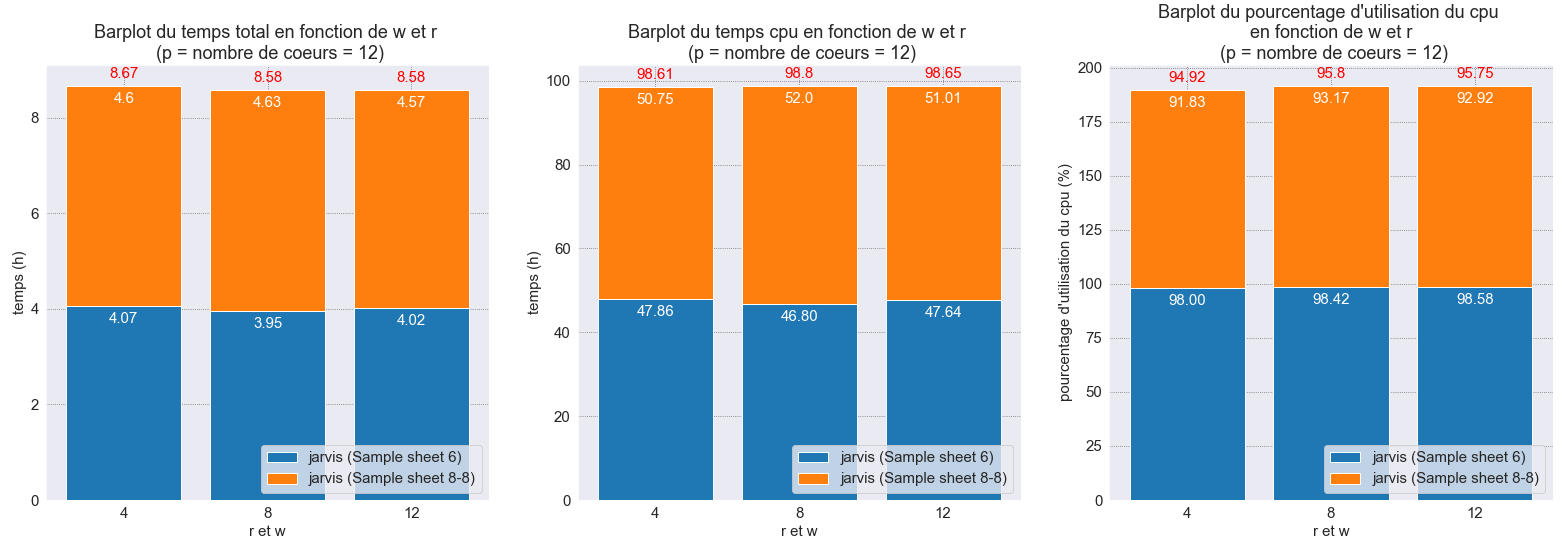
\includegraphics[width=0.8\textwidth]{img/barplot_cum_jarvis2.png}
    \caption{\footnotesize{Digrammes en bâtons du temps total d'éxécution (à gauche), temps cpu (au milieu) et du pourcentage d'utilisation des cpu (à droite) en fonction des paramètres r et w}}
    \label{barplot-param}
\end{figure}

Il y a deux \emph{sample sheet}\footnote{Fichier contenant les informations et instructions pour la génération des fastq et le démultiplexage}, car le nombre de bases considérées des \emph{reads index} entre les \emph{lanes} est différent, obligeant à réaliser deux appels différents au logiciel pour générer les fastq et le démultiplexage. Ci-dessous, la figure \ref{barplot-param2}, représente les résultats obtenus en faisant varier p et en fixant les paramètres r et w à 4 (ces deux paramètres sont fixés à 4 pour pouvoir comparer les 4 résultats). On observe que plus on augmente le nombre de cours et le nombre de \emph{threads} pour p, plus l'execution est rapide. On observe que le temps cpu augmente bien avec le nombre de cœurs et que le pourcentage d'utilisation des cpu est optimal (> 90\%).

\begin{figure}[H]
    \centering
    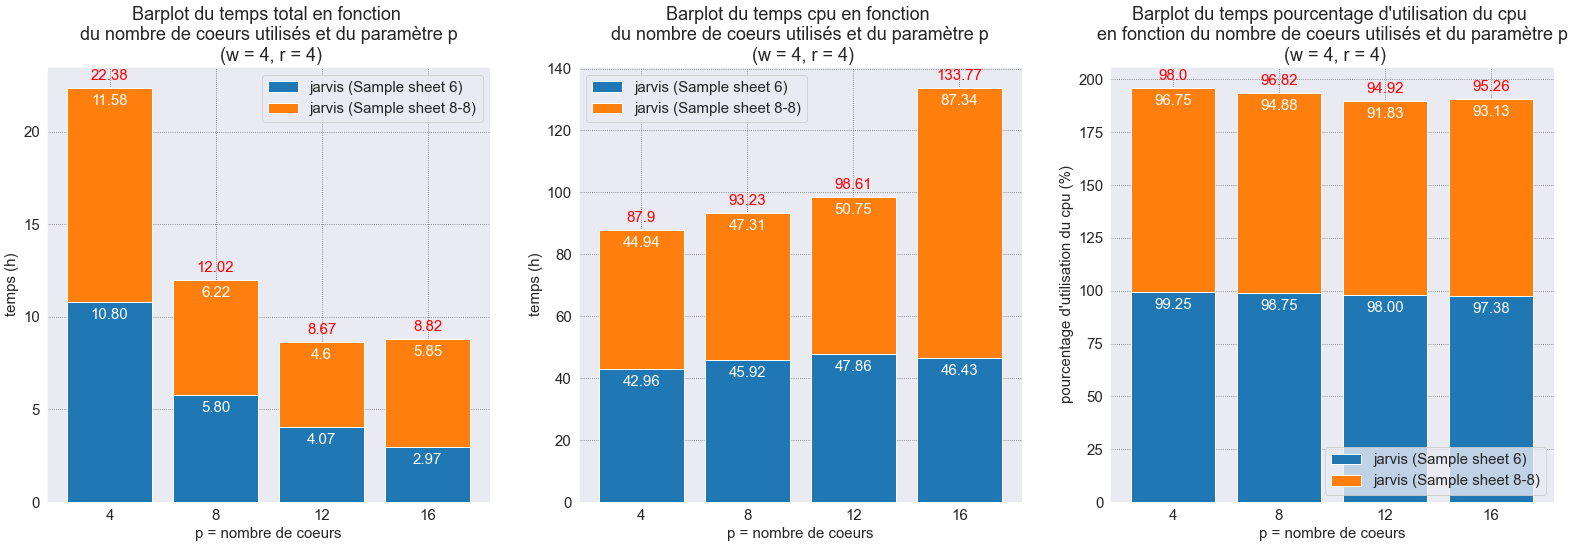
\includegraphics[width=0.8\textwidth]{img/barplot_cum_jarvis1.png}
    \caption{\footnotesize{Digrammes en bâtons du temps total d'éxécution (à gauche), temps cpu (au milieu) et du pourcentage d'utilisation des cpu (à droite) en fonction du paramètre p}}
    \label{barplot-param2}
\end{figure}

Au vue des résultats obtenus nous avons décidé que les meilleurs paramètres étaient de fixer p à 12, puisque le gain apporté en augmentant à 16 est faible. Néanmoins nous le conserverons pour réaliser la comparaison avec bcl-convert, tout comme p fixé à 8, car il nous permettrait de réaliser deux générations de fastq et de démultiplexage en simultané sur un seul noeud de calcul.\\

\subsubsection{Comparaison entre bcl2fastq et bcl-convert}
J'ai donc fait varier les paramètres \texttt{p}, \texttt{r} et \texttt{w} de manière à ce que chacun des paramètre soient égale au nombre de cœurs accordés aux deux logiciels. On observe bien, sur la figure \ref{fig-total-time}, que plus on augmente le nombre de cœurs pour chacun des logiciels (et donc le nombre de \emph{threads} pour \texttt{p}, \texttt{r} et \texttt{w}) plus la génération des fastq et le démultiplexage est rapide. De plus on remarque que bcl-convert permet de réduire le temps d'environs 1/3 par rapport à bcl2fatq. 

\begin{figure}[H]
    \centering
    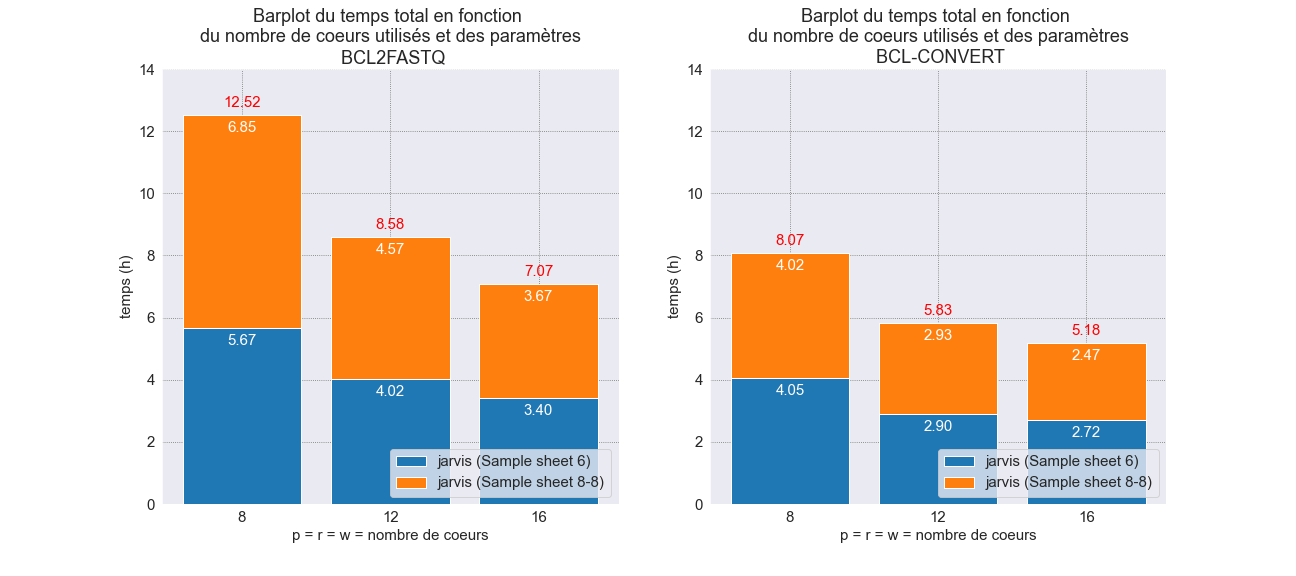
\includegraphics[width=1\textwidth]{img/barplot_total_time_comp.png}
    \caption{\footnotesize{Temps total de génération des fastq pour bcl2fastq et bcl-convert}}
    \label{fig-total-time}
\end{figure}

J'ai également échangé avec le service technique d'Illumina à propos des fichiers de sortie et de l'arborescence de bcl-convert. En effet il s'avère que l'arborescence et les fichiers de sortie sont très différents entre les deux logiciels. Ces échanges avaient pour objectif de savoir s'il on pouvait obtenir une arboresnce similaire à bcl2fastq, pour minimiser l'impact du changement de logiciel sur les pipelines. Le changement de bcl2fstq, qui sera bientôt obsolète, par bcl-convert va nous obliger à réaliser de gros changements dans tous les pipelines qui utilisent ces fichiers de sortie et va demander aussi au laboratoire de séquençage de s'adapter à la nouvelle \emph{sample sheet} de bcl-convert.

\subsubsection{Migration de bcl2fastq vers bcl-convert}
Le logiciel bcl-convert étant plus rapide d'environ 1/3 par rapport à bcl2fastq et que ce dernier sera bientôt obsolète. Sachant également, que le nombre de coeurs disponible par noeuds pour la partition \og \emph{production} \fg{}du cluster de calcul est de 16 coeurs. Nous avons décidé t'attribuer l'intégralité des coeurs d'un noeud de \og\emph{production} \fg{}, c'est à dire 16 coeurs. L'intégralité des changement entre les deux logiciels a été consignés dans un cahier des charges. Il contient, la commande à lancer pour réaliser le \emph{Base Calling}, les modules à charger dans l'environement, le chemin relatif des fichiers de sorties, ainsi qu'un exemple d'arborescence des fichiers de sorties. Ce qui permettera au développeur qui ce chargera de cette migration de suivre ce cahier des charges et ainsi faciliter la migration. Dû à la pression actuelle autour de la technologie MGI, c'est un autre développeur qui sera en charge de réaliser cette migration.

%==============================================================================%
%==============================================================================%

\subsection{Le pipeline de génération de fichiers de séquences pour la technologie MGI}
L'objectif du pipeline NGS\_RG\_MGI est de générer et distribuer les fichiers de séquences dans le bon répertoire de projet, d'échantillon, de type de séquençage et de run.
Tout en créant et mettant à jour les runs, pistes et readsets.
Notament concernant les métriques d'évaluations des ces derniers.
Le pipeline est composé de plusieurs grandes étapes.

\subsubsection{Création et insertion des métriques du run et des pistes dans NGL }
La première étape consite à créer le run et ses pistes dans la base de données NGL, en y intégrant les métriques permettant d'évaluer le run et les pistes (figure \ref{NGL-screenshot_run-lane}).
Le nom du run est constitué de la date de séquençage, le nom du séquenceur et l'identifiant de la flowcell du run.

\begin{figure}[H]
    \centering
    \fbox{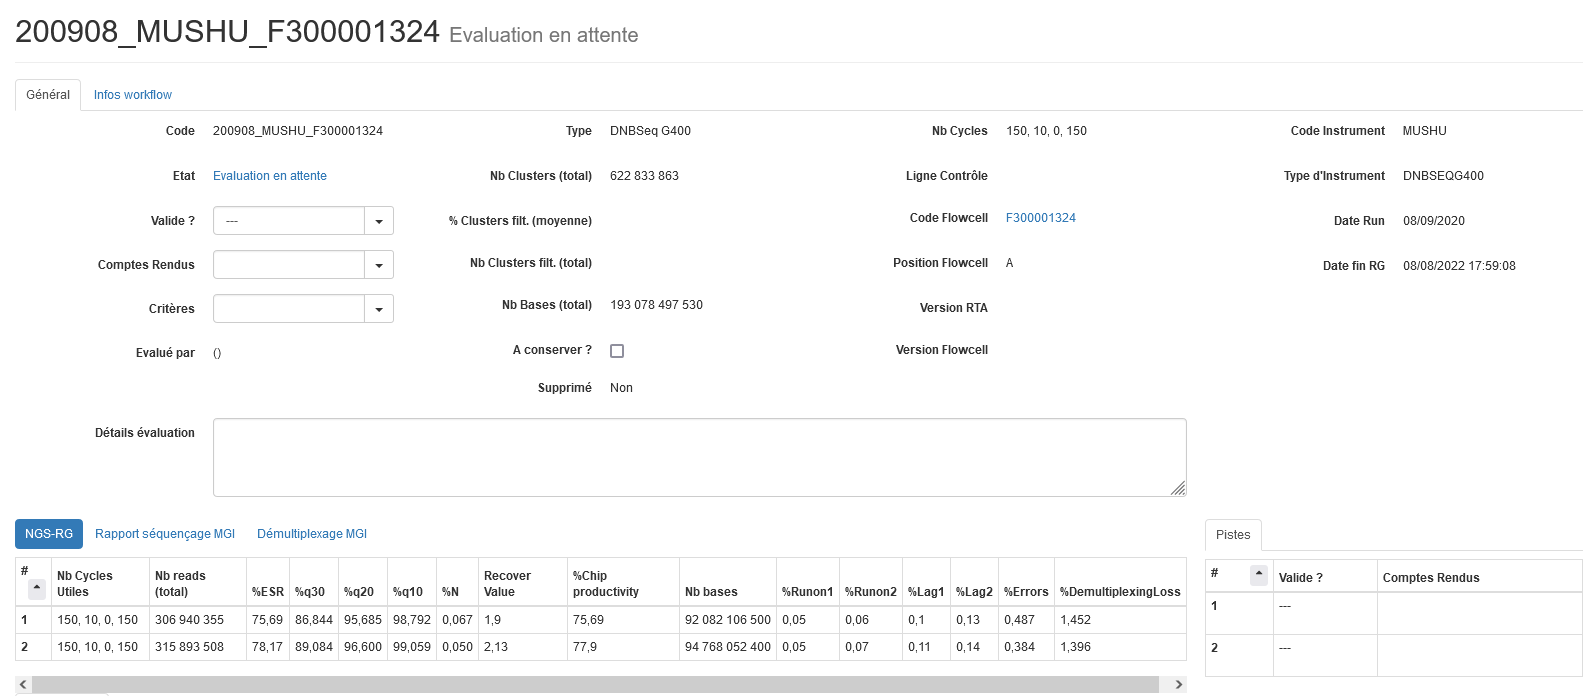
\includegraphics[width=0.9\textwidth]{img/NGL-screenshot_run-lane-ngsrg.png}}
    \caption{\footnotesize{Capture d'écran de la page du run 200908\_MUSHU\_F300001324 de NGL en cours de génération de fichiers de séquences (étapes d'ajout des métriques d'évaluation du run et des pistes).}}
    \label{NGL-screenshot_run-lane}
\end{figure}

On y retrouve notament, le nombre total de reads (Nb Cluster (total)), le nombre de bases totales (Nb Bases (total)) générées par le run, la taille des reads et des index (Nb Cycles).
Concernant les pistes on retrouve le nombre total de bases et de reads générés sur la piste, le pourcentage de bases qui ont une qualité supérieur ou égale à Q30, Q20 et Q10. On a également le pourcentage de bases inconnus (\%N), ainsi que d'autres métriques qui permettent d'avaluer le run et les pistes. Celles-ci sont détaillées plus précisement en anexes (page \pageref{anexes1}).\\

\subsubsection{Insertion des rapports de séquençage des pistes et de la listes des index dans NGL}
La seconde étape ajoute les rapports de séquençages des pistes que le séquenceurs génére en fin de séquençage.
Il s'agit de rapport html qui contiennent plusieurs tableaux de métriques et de graphiques permettant d'évaluer les pistes du run.
Il ya notament les graphiques de la distribution dela qualité moyenne en fonction des cycles (figure \ref{Graph-rapport-pistes}\textcolor{blue}{.A}), de la distribution des bases nucléiques en fonction des cycles (figure \ref{Graph-rapport-pistes}\textcolor{blue}{.B}), de la distribution du pourcentage de Guanine/Cytosine en fonction des cycles (figure \ref{Graph-rapport-pistes}\textcolor{blue}{.C}), de la distribution de l'intensité brut au cours des cycles (figure \ref{Graph-rapport-pistes}\textcolor{blue}{.D}) et d'autres graphiques détaillés en annexes (page \pageref{anexes2}).

\begin{figure}[H]
    \centering
    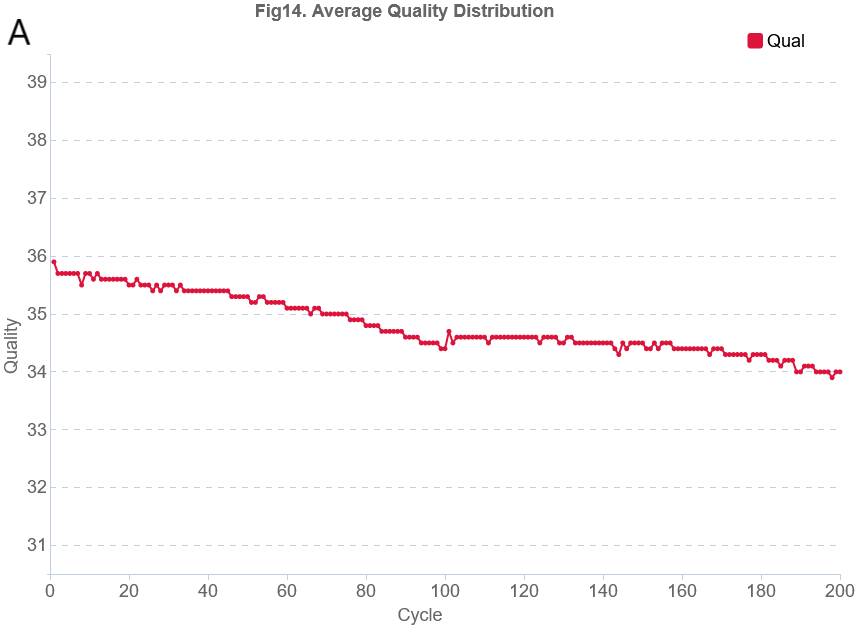
\includegraphics[width=0.48\textwidth]{img/mean_quality.png}
    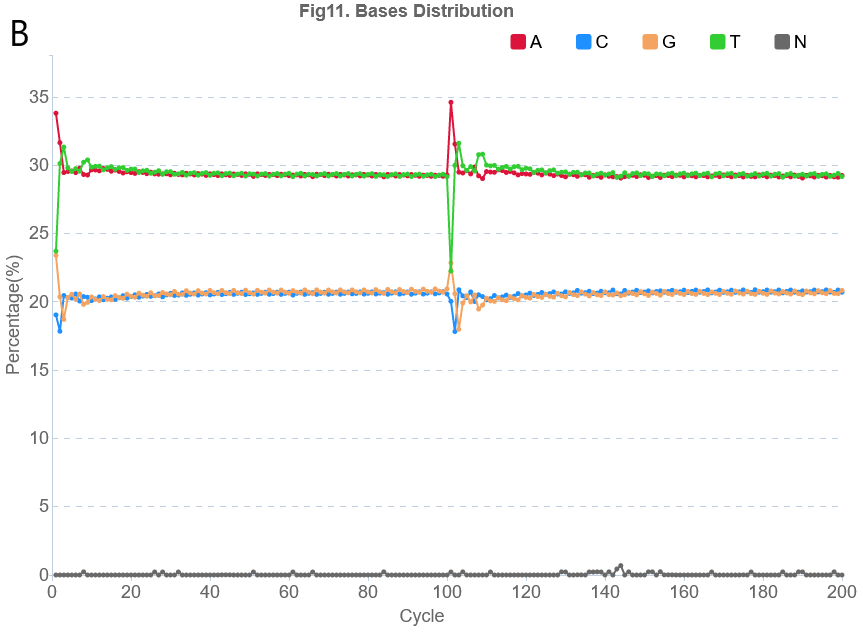
\includegraphics[width=0.48\textwidth]{img/bases_content.png}\\
    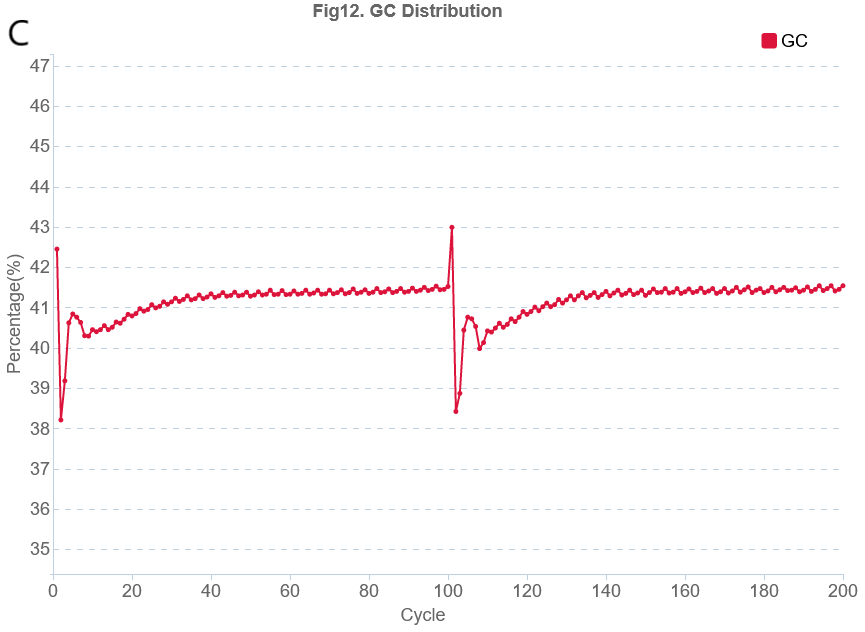
\includegraphics[width=0.48\textwidth]{img/GC_content.png}
    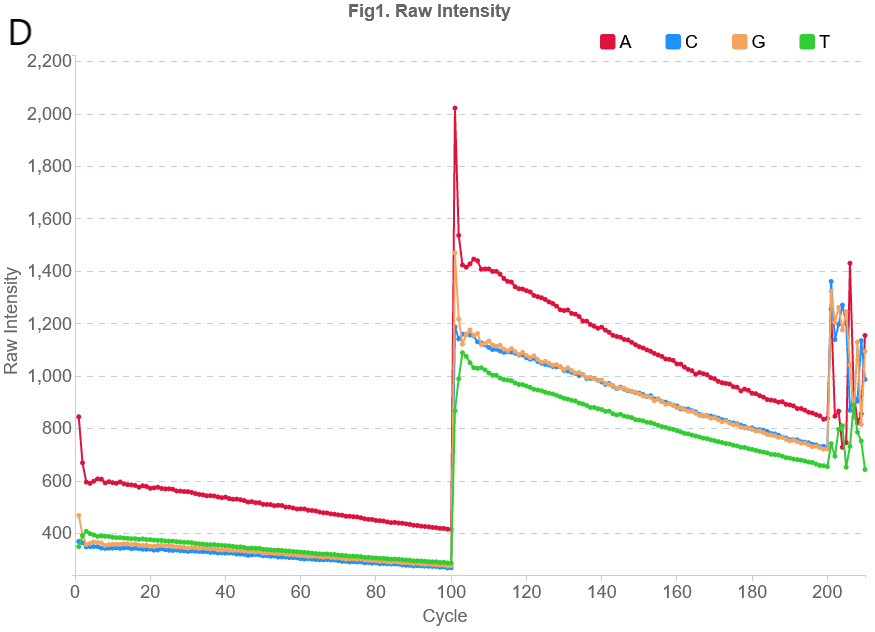
\includegraphics[width=0.48\textwidth]{img/raw_intensity.png}
    \caption{\footnotesize{Graphiques des distributions de la qualité moyenne (A), des bases nucléiques (B), du pourcentage de GC (C) et de l'intensité brut (D) au cours des cycles de séquençage}}
    \label{Graph-rapport-pistes}
\end{figure}

Les tableaux et graphiques de ces rapports de séquençage permettent de facilité l'évaluation du run et de ses pistes.
Toujours dans l'optique de facilité l'évaluation du run et de ces pistes on ajoute, en troisième étape du pipeline, la liste des index représentée à plus de 0.01\% de la pistes, ainsi que les index attendus.
Ces index sont triés et affichés par ordre croissant dans NGL (figure \ref{top-index}).
Les index attendus sont colorés en vert et les index non-attendus ou inconnus sont colorés en rouge, ce qui permet de vérifier que les index attendus sont bien majoritairement représentés sur les pistes de la flowcell du run.

\begin{figure}[H]
    \centering
    \fbox{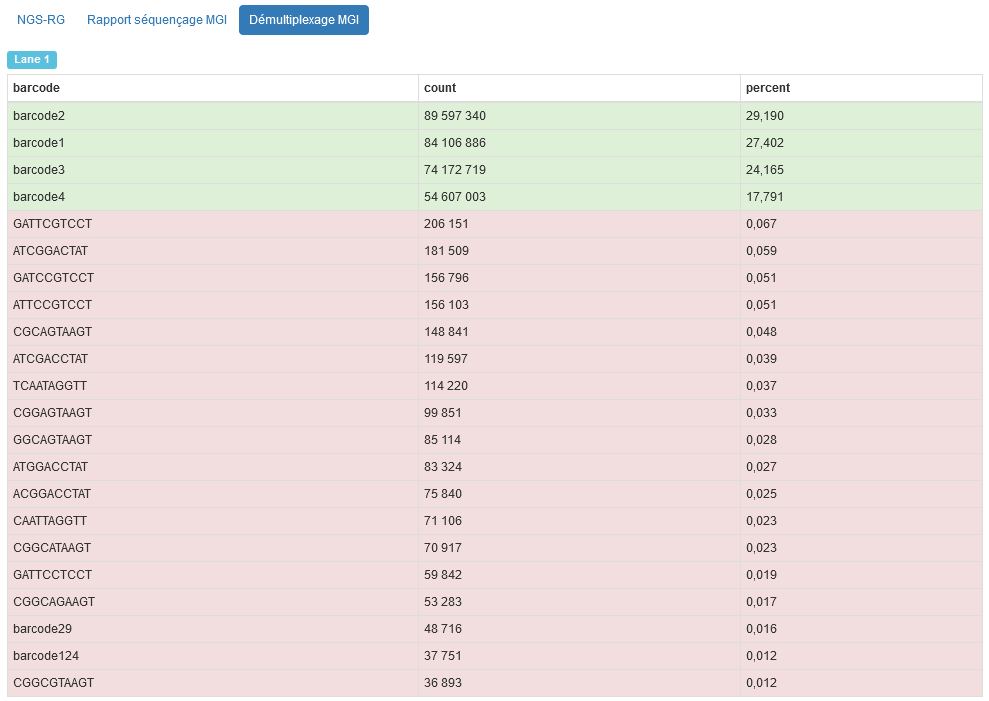
\includegraphics[width=1\textwidth]{img/Top_index.png}}
    \caption{\footnotesize{Capture d'écran de la page du run 200908\_MUSHU\_F300001324 de NGL en cours de génération de fichiers de séquences (onglet \og Démultiplexage MGI\fg{})}}
    \label{top-index}
\end{figure}

\subsubsection{Concaténation des fichiers FASTQ d'un même readset}
Ensuite la quatrième étapes à pour objectif d'obtenir un seul fichier FASTQ par readset.
En effet la technologie MGI requiert une homogénéité de dépôt entre les différents index (aussi appelé\og barcode\fg{}) d'une piste.
Ce qui implique qu'il est possible d'avoir plusieurs index associés à un même index, donc qu'un échantillon peut être divisé en plusieurs fractions.
Le démultiplexage est directement réalisé par le séquenceur, il réalise le démultiplexage à partir des index connus (listes d'index fournis par MGI), on obtient donc un fichier FASTQ par index. Il est impossible de préciser au séquenceur quels index sont associés à un même readset pour le démulitiplexage.
Cette étape est donc essentielle pour obtenir un seul fichier FASTQ par readset.
Si le readset est associé à un seul readset alors on réalise une décompréssion du fichier FASTQ, si le readset est associé à plusieurs index alors on réalise une décompréssion et une concaténation des fichiers FASTQ, tout en le renommant dans un répertoire temporaire (cf. figure \ref{schema-concat-fastq}).

\begin{figure}[H]
    \centering
    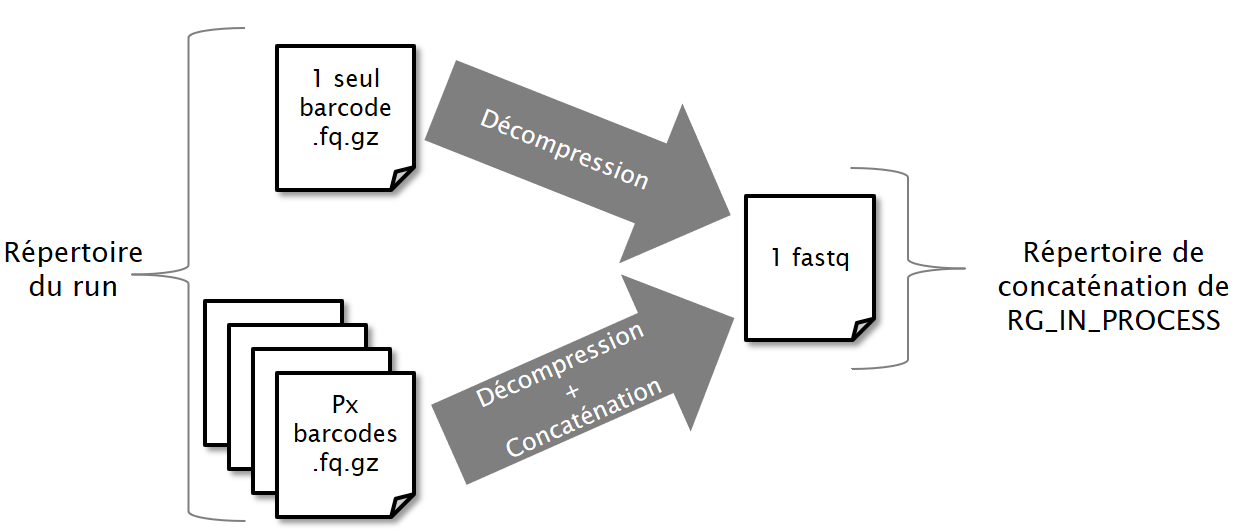
\includegraphics[width=0.6\textwidth]{img/Schéma_concaténation.png}
    \caption{\footnotesize{Schéma de l'étape de \og concaténation\fg{} des fichiers FASTQ d'un readset}}
    \label{schema-concat-fastq}
\end{figure}

\subsubsection{Création et insertion des métriques des readset du run dans NGL}
La cinquiéme étape a pour objectif de permettre l'évaluation des readsets, en les créant et en insérant les métriques d'évaluation de ces derniers dans NGL (figure \ref{NGL-screenshot_readset}).
On y retrouve notamament le nombre de bases nucléiques et de reads du readset, ainsi que le pourcentage d'échantillon déposé sur la piste et le pourcentage de séquences valides par rapport au nombre total de séquences de la piste.
On y insère également certaines métriques du run dont le readset fait partie, comme le nombre de cycles des reads et des index, la date de run, ect. Toutes ces métriques sont décrites en annexes (page \pageref{anexes3})

\begin{figure}[H]
    \centering
    \fbox{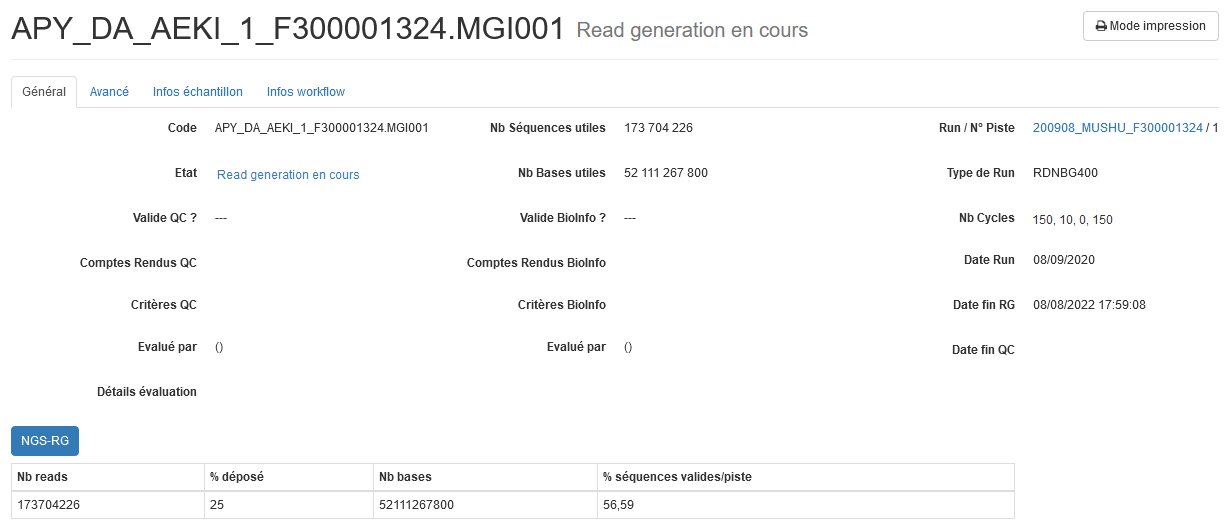
\includegraphics[width=1\textwidth]{img/NGL-screenshot_readset-ngsrg.png}}
    \caption{\footnotesize{Capture d'écran de la page du readset APY\_DA\_AEKI\_1\_F300001324.MGI001 de NGL en cours de génération de reads (étapes de création du readset et d'insertion de ces métriques d'évaluation)}}
    \label{NGL-screenshot_readset}
\end{figure}

Le nom du readset est condstitué de l'identifiant de projet, de l'identifiant du type de banque utilisée (ADN, ARN \dots), de l'identifiant d'échantillon, de l'indice de la lane, de l'identifiant de la flowcell et de l'identifiant du premier barcode.
On ajoute également la répartition des index au sein d'un readset (figure \ref{NGL-screenshot_readset-index}), ce qui permet de vérifier la composition en index du readset et de vérifier l'homogénéité de ces index au sein du readset.
Ce nom de readset est unique, ce qui permet de déterminer rapidement et simplement à quel projet, échantillon, ect appartiennent les fichiers séquences de ce readset.

\begin{figure}[H]
    \centering
    \fbox{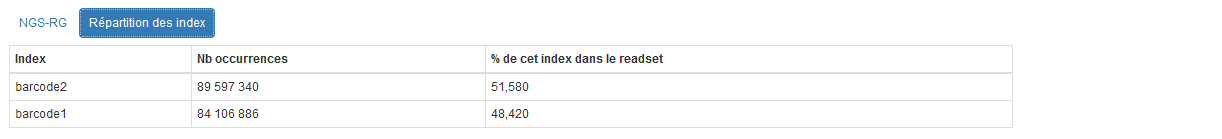
\includegraphics[width=1\textwidth]{img/NGL-screenshot_readset-index.png}}
    \caption{\footnotesize{Capture d'écran de la page du readset APY\_DA\_AEKI\_1\_F300001324.MGI001 de NGL en cours de génération de reads (onglet \og Répartition des index\fg{})}}
    \label{NGL-screenshot_readset-index}
\end{figure}

Au niveaux du run un tableau référençant les readsets et leurs métriques d'évaluation est également ajoutés (figure \ref{NGL-screenshot_tab-run-readset}).

\begin{figure}[H]
    \centering
    \fbox{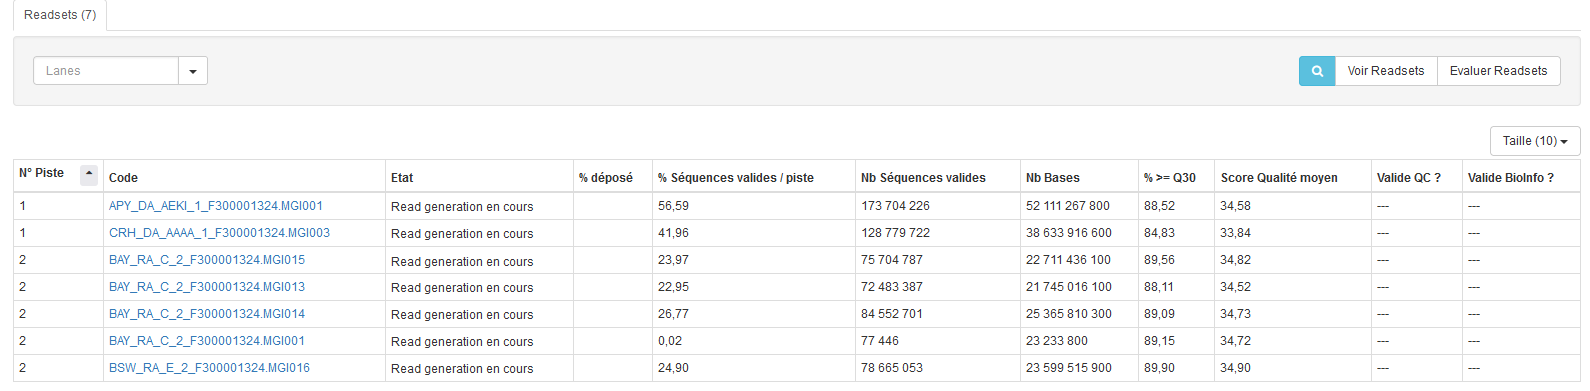
\includegraphics[width=1\textwidth]{img/NGL-screenshot_Tab-readset-in-run.png}}
    \caption{\footnotesize{Capture d'écran de la page du run 200908\_MUSHU\_F300001324 de NGL en cours de génération de fichiers de séquences (Tableau des readset du run)}}
    \label{NGL-screenshot_tab-run-readset}
\end{figure}

\subsubsection{Renommage des fichiers séquences et insertion des méta-données dans NGL}
La sixième étape consiste à renomer les fichiers de séquences des readsets et d'insérer les méta-données de ces derniers dans NGL (figure \ref{meta-data-fastq}).
Le renommage des fichiers est nécessaire pour que chaque fichier de séquence ait un nom unique et \og parlant\fg{}.\\

\begin{minipage}{0.45\textwidth}
    \begin{figure}[H]
        \centering
        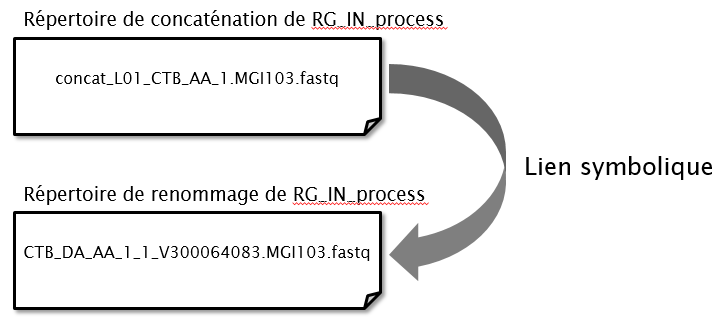
\includegraphics[width=1\textwidth]{img/Schema-renomage-fastq.png}
        \caption{\footnotesize{Schéma de l'étape de renommage des fichiers FASTQ d'un readset}}
        \label{schema-rename-fastq}
    \end{figure}
\end{minipage}
\hfill
\begin{minipage}{0.45\textwidth}
    Le nom doit permettre d'indentifier rapidement et simplement de quel projet, échantillon, flowcell, ect.
    appartient le fichier.
    Le renomage des fichiers est effectué en créant un lien symbolique des fichiers obtenus à l'étape de \og concaténation\fg{} dans un répertoire temporaire (cf figure \ref{schema-rename-fastq}).
\end{minipage}\\

Les méta-données, des fichiers de séquences du readset, qui sont insérées dans NGL permet aux utilisateurs de trouver rapidement l'emplacement de ces derniers sur le système de fichier, le type de fichier disponible (brut, nettoyer) et s'ils sont utilisable.
On y retrouve donc le chemin vers le repertoire de ces fichiers, leurs noms, leurs types, s'ils sont utilisable, s'il s'agit du read \emph{forward} ou \emph{reverse}, et le type d'encodage de la quality (Pour les séquenceurs MGI l'encodage est en ASCII 33).

\begin{figure}[H]
    \centering
    \fbox{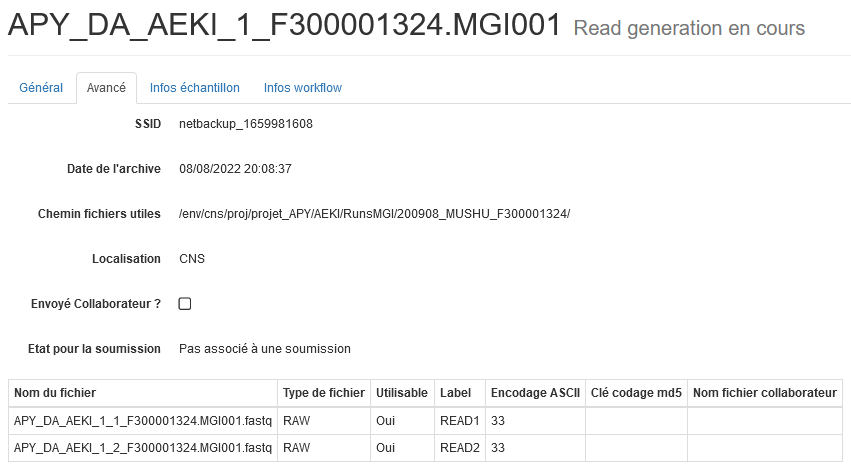
\includegraphics[width=1\textwidth]{img/meta-data-fastq.png}}
    \caption{\footnotesize{Capture d'écran de la page du readset APY\_DA\_AEKI\_1\_F300001324.MGI001 de NGL en cours de génération de fichiers de séquences (Onglet \og Avancé\fg{})}}
    \label{meta-data-fastq}
\end{figure}

\subsubsection{Distribution des Fichiers séquences et des fichiers de statistiques}
La septième étape est de distribuer des fichiers de séquences \og attendus\fg{}, les fichiers de statistiques du run et les fichiers de séquences \og non attandus\fg{} dans leurs répertoires dédiés.
Les fichiers attendus sont copiés vers leurs répertoires finales si le séquençage a été effectué au genoscope.
Si ce dernier a été effectué au CNRGH, alors les fichiers sont copié et compressés.
Il y a cette différence entre les 2 centres, car le pipline de contrôle qualité prend en charge de fichiers compressés pour le CNRGH, contrairement à celui utilisé pour le Genoscope.

Les fichiers de statistiques du run sont archivés par pistes et par types (.html, .fq.stat) avant d'être copié vers leurs répertoires finales.
Ces fichiers sont conservés dans le cas où une métrique désirés ne fait pas partie de celles insérées dans NGL ou pour tout autres probléme qui nécéssiterait de récupérer les fichiers de statistiques du run.

Concernant les fichiers \og non attendus \fg{}, il s'agit des fichiers de séquence des index ne faisant pas partie d'un readset. Puisque lors du demultiplexage par les séquenceurs, on obtient un fichier FASTQ par index.
Ces fichier sont renomés et archivés, avant d'être distribués vers leur répertoire dédiés.
Ces fichers de séquences sont conservés dans l'éventualité d'une mauvaise déclaration d'index par les équpies de séquençage, pour pouvoir récupérer les fichiers fastq appartenant à cet index ou si l'on souhaite étudier les séquences des fichiers \og non-attendus\fg{}.\\

\subsubsection{Mise à jour de fin de génération de fichiers de séquence dans NGL}
L'étape finale du pipeline de génération de fichiers de séquences pour la technologie MGI, est de mettre à jour le run et les readset dans l'état de \og fin de génération de reads\fg{}.
Cela entraine une mise à jour automatique du run à l'état \og d'évaluation en attente\fg{}, ce qui permet d'indiquer aux utilisateurs que le run peut être évalué.
Les readset sont aussi automatiquement mis à jour vers l'état \og d'attente de contrôle qualité\fg{}, permettant d'indiquer au pipeline de contrôle qualité qu'il peut effectuer le contrôle qualité des readset de ce run.


\input{sections/discutions.tex}
\section{Perspectives}

\subsection{Workflow MGI}
Concernant le workflow de MGI, il nous faut dans un premier temps déterminer les outils et méthodes necessaires (utilisation de ceux du workflow d'Illumina ou de nouveaux). Une fois ceci déterminé il restera à écrire les deux pipelines, celui de génération de reads (ngs\_rg\_mgi) et celui de contrôle qualité (ngs\_rg\_mgi). L'objectif sur le long terme est d'arriver à un workflow totalment automatisé, comme celui d'Illumina.\\

\subsubsection{Le pipeline NGS\_RG\_MGI}
\textcolor{red}{ajout démidage, maintient pipeline. ??????????}

\subsubsection{Le pipeline NGS\_QC\_MGI}
\textcolor{red}{maintient pipeline. ?????????}

\subsection{Évaluation d'outils}
Il y aura aussi l'évaluation d'autres outils utiles pour les pipelines, comme des outils de \emph{trimming}, \emph{filtering}, d'assignation taxonomique, etc.

\newpage
\addcontentsline{toc}{section}{Notes}
\theendnotes
%=============================================================================%
%============================= reférences ====================================%
\newpage
\addcontentsline{toc}{section}{Références}
\bibliographystyle{abbrv}
\bibliography{biblio}
\nocite{*}
%=============================================================================%
%		      				Fin document		  							  %
%=============================================================================%
\end{document}



























\begin{minipage}{0.45\textwidth}
	\begin{figure}[H]
		\centering
		\includegraphics[width=1\textwidth]{img/optimal_clusters_HCA.png}
		\caption{Détermination graphique du nombre de clusters optimal pour la classification à l'aide de HCA}
		\label{fig3}
	\end{figure}
\end{minipage} 
\hfill
\begin{minipage}{0.5\textwidth}
	\begin{figure}[H]
        \centering
        \includegraphics[width=1\textwidth]{img/heatmap.png}
        \caption{Heatmap de la classification des poches et des descripteurs par HCA}
        \label{fig4}
    \end{figure}
\end{minipage}

\begin{figure}[H]
    \centering
    \includegraphics[width=0.45\textwidth]{img/poucentage_variance_composante_pca.png}
    \includegraphics[width=0.45\textwidth]{img/pca_biplot_hca.png}
    \caption{Détermination graphique du nombre de composante nécessaire (à gauche) et visualisation des clusters sur les 2 premières composantes de l'ACP (à droite)}
    \label{fig5}
\end{figure}